\chapter{Modelling of Devices}
\label{secModellingDevices}

\begin{table}[bt]
\begin{center}
\begin{tabular}{|p{2.8cm}|p{2.5cm}|p{2.9cm}|p{5.9cm}|} % 14.3cm in total available

\hline

% The column headers:
Device & Known quantity & Unknown quantity & Meaning \\
\hline
% The next hline makes the column titles a separate rectangular box,
% comment it out to get just a line as separator.
%\hline

\hline

% Table entries start here.

Node & - & \ident{U\_$<$nameOfNode$>$} & Voltage potential of node.
There's no such unknown for the ground node \\
\hline

Passive device & - & - & Passive devices, R, Y, C and L, don't introduce
knowns or unknowns to the LES. They only appear as symbols in the computed
results \\
\hline

Constant voltage source & \ident{$<$nameOfDev$>$} & - & Given voltage of
source; 1st connected node is plus pole \\
\hline

Constant current source & \ident{$<$nameOfDev$>$} & - & Given current through
source flowing from 1st to 2nd connected node \\
\hline

Op-amp & - & \ident{I\_$<$nameOfDev$>$} & Output current of op-amp. The current
flows from ground node to output node, then into the network\\
\hline

Voltage controlled voltage source & - & \ident{I\_$<$nameOfDev$>$} &
Current through source flowing from 2nd to 1st connected node \\
\hline

Current controlled voltage source & - & \ident{I\_$<$nameOfDev$>$} &
Current through source flowing from 2nd to 1st connected node \\
\hline

Voltage controlled current source & - & \ident{I\_$<$nameOfDev$>$} &
Current through source flowing from 1st to 2nd connected node \\
\hline

Current controlled current source & - & \ident{I\_$<$nameOfDev$>$} &
Current through source flowing from 1st to 2nd connected node \\
\hline

Current probe & - & \ident{I\_$<$nameOfDev$>$} or \ident{$<$nameOfDev$>$}
& Measured current flowing through probe from 1st to 2nd connected
node.

The prefix \ident{I\_} in the name of the unknown current is omitted
if the probe's name already begins with \ident{I\_} (case sensitive
comparison) \\
\hline

\end{tabular}
\caption{Knowns and unknowns of the LES. These quantities can be
referenced in user-defined results}
\label{tabUnknownsOfLES}
\end{center}
\end{table}


A linear electronic circuit is modeled by \linnet{} as a system of linear
equations. These equations basically describe the current balances at the
nodes: since the nodes are conceptually free of the capabilty of storing
charge all influent currents are in sum at any time equal to the sum of
affluent currents. If the flow direction is expressed by a current's sign
than this statement is simplified to the sum of currents is null at any
time. This is applied to most of the nodes and gives us a number of
equations.

If we have $N$ nodes then we can make this statement mostly only for $N-1$
of them; the current balance of the last node would become linear
dependent, or with other words, the last equation would just be a weighted
sum of the others.

The currents flowing in or out of the node in question are determined by
the devices connected to this and neighboured nodes. The voltage
potentials of the nodes become the unknowns of the equation system and the
flowing currents can be expressed as functions of these potentials. Doing
this consequently for all devices completes the equations or yields the
full set of coefficients of the equation system in its matrix
representation.

A netlist can describe a circuit, which are actually two, three or more
unconnected sub-circuits. Here, unconnected means that there's no wired
connection between the sub-circuits. The sub-circuits may but don't need
to be logically independent; there may be logical interdependencies as
introduced by controlled sources: the source is in one sub-circuit but
the controlling voltage or current is found in another one. Reasonable
use-cases are known, which result in such logically dependent but
unconnected sub-circuits in a netlist.

If there are unconnected sub-circuits -- regardless whether logically
coupled or completely irrelated -- then the number of equations expressing
the current balances of nodes is further reduced; in general there will be
one dependent equation per sub-circuit.

A voltage is always defined as the difference of two voltage potentials,
in our application the voltage potential difference between two nodes
only. The last, dependent node of any sub-circuit is called the ground
node and gets the arbitrary voltage potential null at any time by
definition. Which means that voltages were even defined between nodes of
different, unconnected sub-circuits, although this is not described by the
schematic and physically undefined. To avoid misleading results, which
were correct only on condition of this definition, \linnet{} refuses the
definition of voltages between nodes in unconnected sub-circuits. This
holds for user-defined voltages and control voltages of voltage controlled
sources.

The terms of the current balance equation of a particular node $N$ are
principally dictated by the linear devices connected to this node as they
conduct the in- and affluent currents but there are also some additional
constraints, mainly introduced by the sources. How the equation system is
build up from the list of devices (i.e. the netlist) is documented in the
next sections. Table \ref{tabUnknownsOfLES} gives an overview on the
knowns and unknowns of the evolving equation system. The quantities listed
in the table can be referenced when specifying a user-defined result in
the netlist file.


\section{Passive devices}

The passive devices are resistor, conductance (actually the same as a
resistor but the device value is defined reciprocal), capacitor and
impedance. All of these devices are characterized by the fact that the
(complex) current is proportional to the (complex) voltage between the two
ends of the device. All of these devices are handled exactely the same,
only a different proportionality factor is considered.

However, the differences in the proportionality factors are considered
only in the final result representation. \linnet{} has a symbolic equation
solver and during the complete elimination process the applied symbol has
the meaning of complex conductance -- whatever this is for the given
device. For all of these devices holds $I_s=s U_s$, if s is the symbol
representing the device. The effective voltage $U_s$ in this equation, the
voltage between the two ends of device $s$, is the difference of the
voltage potentials of the nodes the device is connected to. The sign of a
current is a matter of definition and \linnet{} defines it to be positive
if it is influent. We get: $I_s=s(U_{n_j} - U_{n_i})$, where $n_i$ is the
node under progress, i.e. the node the current balance is made for and
$n_j$ is the other node the device is connected to. If these terms are
taken for all devices, which are connected to node $n_i$ than the current
balance of this node is widely done for this node; the other side of the
equation simply is a null.

\begin{figure}
  \centering
  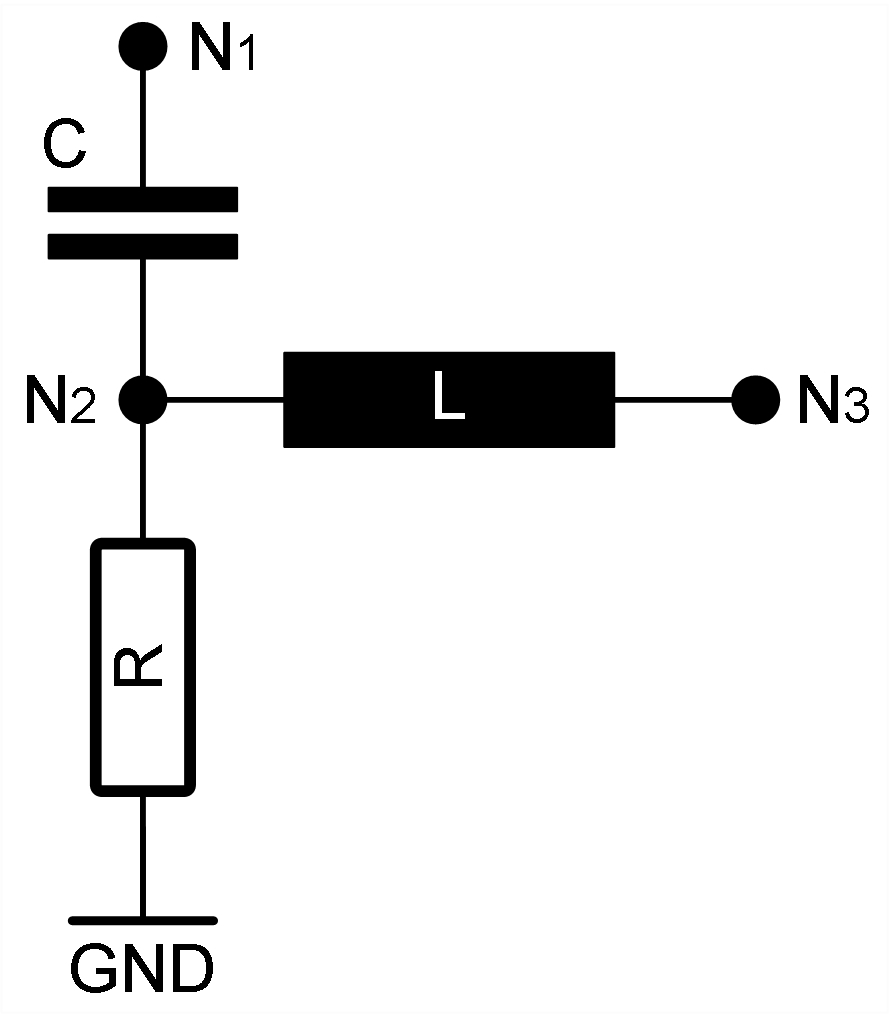
\includegraphics[width=3cm]{LESCreation_fragmentOfPassiveDevices}
  \caption{Fragment of circuit, handling of passive devices}
  \label{figLESCreation_fragmentOfPassiveDevices}
\end{figure}

As usual, the equation system is represented by a matrix. This means only
the coeffcients of the equations are actually represented, the product
with the unknowns $U_{n_j}$ and $U_{n_i}$ is implicit. Which means that
``take a term'' just means to put the symbol $s$ twice in the row of the
matrix, which represents the current balance of node $n_i$: in column $j$
(assuming that this column represents unknown $U_{n_j}$) and as $-s$ in
column $i$ (assuming that this column represents unknown $U_{n_i}$).

The same is repeated for all independent nodes in the circuit. The same
symbol $s$ will appear again, when the process visits node $n_j$. This
time the perspective is inverse and symbol $s$ will appear with inverse
signs in the row that represents the current balance of node $n_j$.

If one of the two nodes the device is connected to should be the ground
node than there is no current balance for this node and one of the two
rows of the matrix containing symbol $s$ will disappear. Same for the
columns, as the ground node's voltage potential doesn't belong to the set
of unknowns. We end up with a single appearance of symbol $s$ in the
matrix.

Figure \ref{figLESCreation_fragmentOfPassiveDevices} shows a fragment of
a circuit. If we assign node $n_i, i=1 \ldots 3$ to row and column $i$ of
our matrix then this fragment would lead to the following matrix:

\begin{displaymath}
\label{eqLESCreation_fragmentOfPassiveDevices}
\left(
\begin{array}{cccc}
-C      & C      &  0     & \ldots \\
 C      & -C-L-R &  L     & \ldots \\
 0      &    L   & -L     & \ldots \\
 \vdots & \vdots & \vdots & \ddots \\
\end{array}
\right)
\end{displaymath}


\subsection{Symbols, knowns and unknowns}

\begin{table}[bt]
\begin{center}
\begin{tabular}{|l|c|p{2cm}|}

\hline

% The column headers:
Kind of device & Substitute of symbol & Meaning \\
\hline
% The next hline makes the column titles a separate rectangular box,
% comment it out to get just a line as separator.
%\hline

\hline

% Table entries start here.
R & \raisebox{0pt}[10pt][5pt]{$\frac{1}{R}$}  & Resistor    \\
Y & $Y$                                       & Conductance \\
L & \raisebox{0pt}[10pt][5pt]{$\frac{1}{Ls}$} & Impedance   \\
C & $Cs$                                      & Capacitor   \\

 \hline
\end{tabular}
\caption{Substitution of symbols in the final result}
\label{tabSubstOfSymbols}
\end{center}
\end{table}

The passive devices don't introduce knowns or additional unknowns to the
equation system.

The name of a device is used as symbol in the internal computation and as
variable in the final result representation. Although it is the same
symbol it has different meanings in either case: In the internal
computation it designates the complex conductance, whereas it has the
common, physical meaning in the final result. For example, $C$ would
actually mean the frequency dependent complex conductivity $Cs$ during the
internal computation but designate the constant, real capacitance in Farad
of a capacitor in the final result.

In the final result representation, the symbols of the internal
computation are substituted by the physical expressions in the complex
frequency variable $s$. This is done according to table
\ref{tabSubstOfSymbols}.

The values for the $R$, $Y$, $L$ and $C$ in the final result, which are
used as default in numeric post-processing with Octave can be found in
table \ref{tabDeviceStdValues} on page \pageref{tabDeviceStdValues}.


\section{Constant voltage source}
\label{secModellingDevs_ConstVoltSrc}

The constant voltage source is a constraint on the LES. The source is
connected to two nodes. These node's voltage potentials, which are both
unknowns to the system are associated by the constraint that they differ
by a constant, given, known voltage.

The constraint is expressed as a simple additional equation, which says
$U_{n_i} - U_{n_j} - U_{ij} = 0$, where $U_{ij}$ is the constant voltage
of the source connected to nodes $n_i$ and $n_j$.

The constant voltage source introduces a further known and thus a further
column to the LES. The additional equation means a further row, too. The
equation is just a triple of signed ones at the according columns. (If the
source is connected to a ground node then only two ones remain.)

The additional equation comes along with an additional unknown. When
setting up the current balance of the connected nodes we have to consider
the additional circuit branch, the current flowing through the source.
This current is unknown. It is defined to be the current flowing out of
the source's plus pole; it's influent and thus positive at the node
connected to the plus pole and affluent or negative at the minus pole's
connetced node. We get a second additional column, which has a pair of
$\pm 1$ as only non null coefficients (or a single signed one if one of
the nodes would be the ground node).

As an example, the source $U_0$ would be connected with its plus and minus
pole between the nodes $N_1$ and $N_3$, respectively, of the circuit
fragment in figure \ref{figLESCreation_fragmentOfPassiveDevices}. The new
unknown current \ident{I\_U0} is put to the right of the unknowns so far
and the new known to the right of the knowns so far. The LES would be
extended to:

\begin{displaymath}
\left(
\begin{array}{ccccccc}
-C      & C      &  0     & \ldots & 1      & \ldots & 0       \\
 C      & -C-L-R &  L     & \ldots & 0      & \ldots &         \\
 0      &    L   & -L     & \ldots & -1     &        & \vdots  \\
 \vdots & \vdots & \vdots &        &        &        & 0       \\
 1      &    0   & -1     & 0      & \ldots & 0      & -1      \\
\end{array}
\right)
\end{displaymath}

Only the constant sources, either voltage or current, introduce the knowns
into the LES. At least one known, hence constant source, is required
otherwise \linnet{} refuses to compute the circuit. The system would
remain unstimulated and all voltages and currents would anyway be null.

If more than one constant source is used then the system changes to a MIMO
system and the result function for an unknown has several terms to
describe the dependency of the unknown on each of the knowns (given a full
results is requested).


\subsection{Symbols, knowns and unknowns}

The source is represented in the LES only as a number of coefficients $\pm
1$ and its name does not appear as a symbol in the internal computation.
It is a known and only apparent in the final result representation. Here,
it has the meaning of the Laplace transform of the given source voltage in
Volt.

The name of the additional unknown, the current through the source is
derived from the device name by adding the prefix \ident{I\_} to the left
of the user-defined device name. The name of the additional unknown does
not appear as a symbol in the internal computation. It can be referenced
in a result specification in order to get an according transfer function
or full result.



\section{Constant current source}

A constant current source is modeled as a known current, which is
influent (i.e. positive) at the node connected to the source's plus pole
and affluent (i.e. negative) at its minus pole's connected node. This
leads to a new column for the additional known, which has just a pair of
$\pm 1$ coefficients at the rows related to the connected nodes (and hence
only a single signed one if one of these nodes is the ground node). All
other coefficients in this column remain null.

As an example, the current source $I_0$ would be connected with its plus
and minus pole between the nodes $N_1$ and $N_3$, respectively, of the
circuit fragment in figure \ref{figLESCreation_fragmentOfPassiveDevices}.
The new known is put to the right of the knowns so far. The LES would be
extended to:

\begin{displaymath}
\left(
\begin{array}{ccccc}
-C      & C      &  0     & \ldots & 1  \\
 C      & -C-L-R &  L     & \ldots & 0  \\
 0      &    L   & -L     & \ldots & -1 \\
 \vdots & \vdots & \vdots &        &    \\
\end{array}
\right)
\end{displaymath}

At least one constant current or voltage source is required otherwise
\linnet{} refuses to compute the circuit; see section
\ref{secModellingDevs_ConstVoltSrc} for more.


\subsection{Symbols, knowns and unknowns}

The source is represented in the LES only as a pair of coefficients $\pm
1$ and its name does not appear as a symbol in the internal computation.
It is a known and only apparent in the final result representation. Here,
it has the meaning of the Laplace transform of the given source current in
Ampere.

The constant current source doesn't add any unknowns to the LES.


\section{The operational amplifier}

% Sample circuit: Op-amp LP 2 times with two different ground nodes
{
% This define is related to the specifics of the array package; see
% http://texwelt.de/wissen/fragen/3401/zentrieren-text-in-tabelle (as of
% July 25 2014) for more
\newcolumntype{M}[1]{>{\centering\arraybackslash}m{#1}}

\begin{figure}[tb]
\begin{center}
\begin{tabular}{M{6cm}M{5.89cm}}
\verbatiminput{OpampLPWithDifferingGnds.cnl}
&
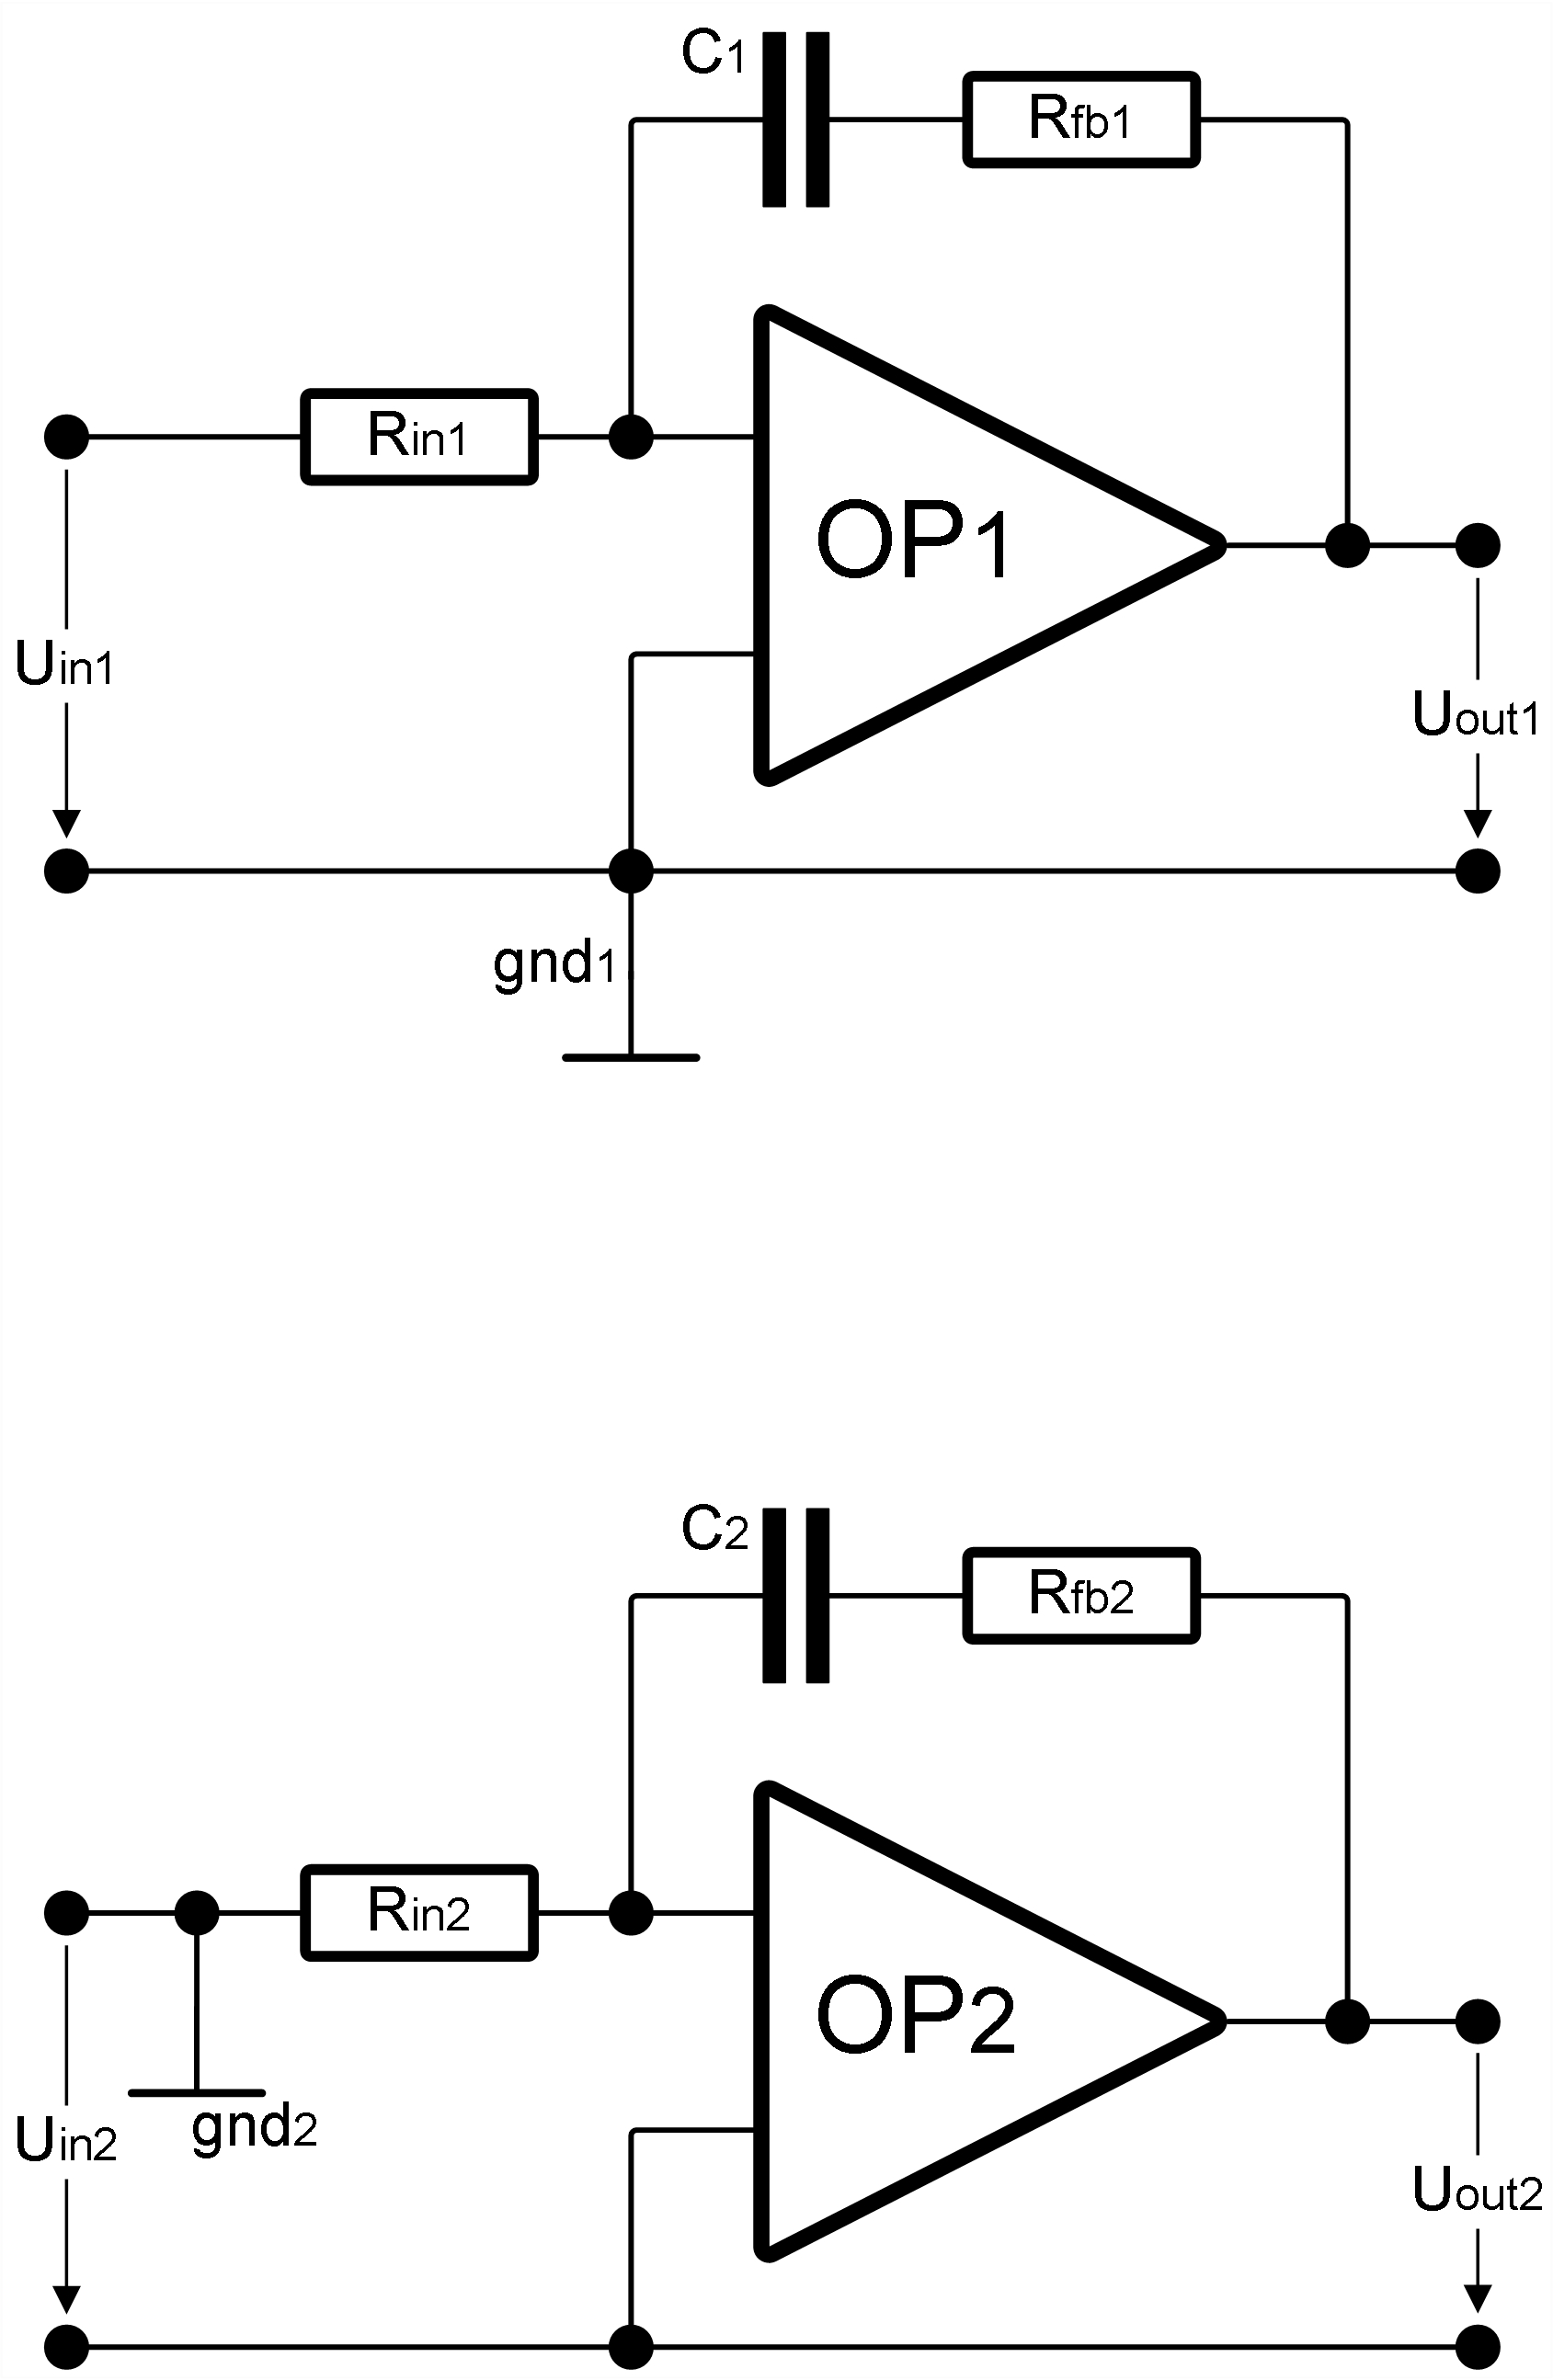
\includegraphics[width=5.89cm]{OpampLPWithDifferingGnds}

\end{tabular}
\caption{Low-pass filter with op-amp and two choices of ground node}
\label{figOpampLPWithDifferingGnds}
\end{center}
\end{figure}
} % Sample circuit: Op-amp LP 2 times with two different ground nodes


Linear operational amplifier circuits are based on the principle, that the
voltage between the two inputs is highly amplified but fed back to one of
the inputs such that the input voltage is compensated till close to null.
The remaining input voltage is in the magnitude of a few micro Volts only
and the output voltage in the magnitude of a few volts. The high dynamic
capabilities of the implementation of the op-amp ensure that this balance
is kept at any time.

The output voltage of the op-amp leads to an output current. This current
is controlled by a push-pull output stage, which lets the output current
flow either from the positive supply voltage or into the negative supply
voltage. (These supply voltages therefore limit the actual output voltage
range.)

The real op-amp is modeled by \linnet{} in an idealized way. The
amplification is made infinite and the feedback by the outer circuitry
thus leads to a voltage of exactely null between the inputs. The dynamic
capabilities become infinitely fast; there's no reaction time, the
equations hold at any time.

Controlling the output voltage by a push-pull output stage is a highly non
linear behavior of the true implementation of an op-amp and can't be
modeled as such by \linnet{}. Instead, \linnet{} approaches this behavior
by a controlled voltage source, which is connected between ground and the
op-amp's output. The voltage is controlled such that the input voltage
becomes null.

Modelling an op-amp like this has several important implications. Most
striking, this model doesn't require any distinction of the two inputs of
the op-amp. The output condition simply is that the input voltage be null;
only the real implementation of the circuitry requires careful selection
of the right input so that the feedback leads to a voltage compensation
rather than to a boost. Contrariwise, any kind of circuit, which founds on
a voltage boost by toggling the inputs (like threshold detector, Schmitt
trigger, etc.) can't simply be modeled with \linnet{}.

Most obvious, there is no output voltage limitation. The output voltage
will raise or drop to any voltage until the condition for the input
voltage is met.

More in general, there is no modelling of the voltage supply at all. Using
an op-amp in \linnet{} only enables to compute the small-signal behavior
of the true circuit; the DC behavior with all supply voltages and currents
and the related power distribution can't be figured out. Furthermore, the
decision to model the output by a voltage source, whose other end is
connected to ground means that the full picture of the solution depends on
the choice of the ground node. An example is given. A low-pass filter is
implemented twice in a single netlist, where the only difference (besides
indexing of the object names) is the different choice of the ground
node. Please refer to figure \ref{figOpampLPWithDifferingGnds}.

\linnet{} computes the same transfer function from input to output voltage
for both variants of the filter. Please compare $U_{out_1}$ with
$U_{out_2}$:

\begin{verbatim}
RESULT - User-defined result G1 (Bode plot):
The dependency of Uout1 on Uin1:
  Uout1(s) = N_Uout1_Uin1(s)/D_Uout1_Uin1(s) * Uin1(s), with
    N_Uout1_Uin1(s) = -Rfb1*C1 * s
                      -1
    D_Uout1_Uin1(s) = Rin1*C1 * s
RESULT - User-defined result Z1 (Bode plot):
The dependency of Uin1 on I_Uin1:
  Uin1(s) = N_Uin1_I_Uin1(s)/D_Uin1_I_Uin1(s) * I_Uin1(s), with
    N_Uin1_I_Uin1(s) = Rin1
    D_Uin1_I_Uin1(s) = 1
RESULT - User-defined result G2 (Bode plot):
The dependency of Uout2 on Uin2:
  Uout2(s) = N_Uout2_Uin2(s)/D_Uout2_Uin2(s) * Uin2(s), with
    N_Uout2_Uin2(s) = -Rfb2*C2 * s
                      -1
    D_Uout2_Uin2(s) = Rin2*C2 * s
RESULT - User-defined result Z2 (Bode plot):
The dependency of Uin2 on I_Uin2:
  Uin2(s) = N_Uin2_I_Uin2(s)/D_Uin2_I_Uin2(s) * I_Uin2(s), with
    N_Uin2_I_Uin2(s) = 1
    D_Uin2_I_Uin2(s) = 0
\end{verbatim}

\begin{figure}[tb]
\begin{center}
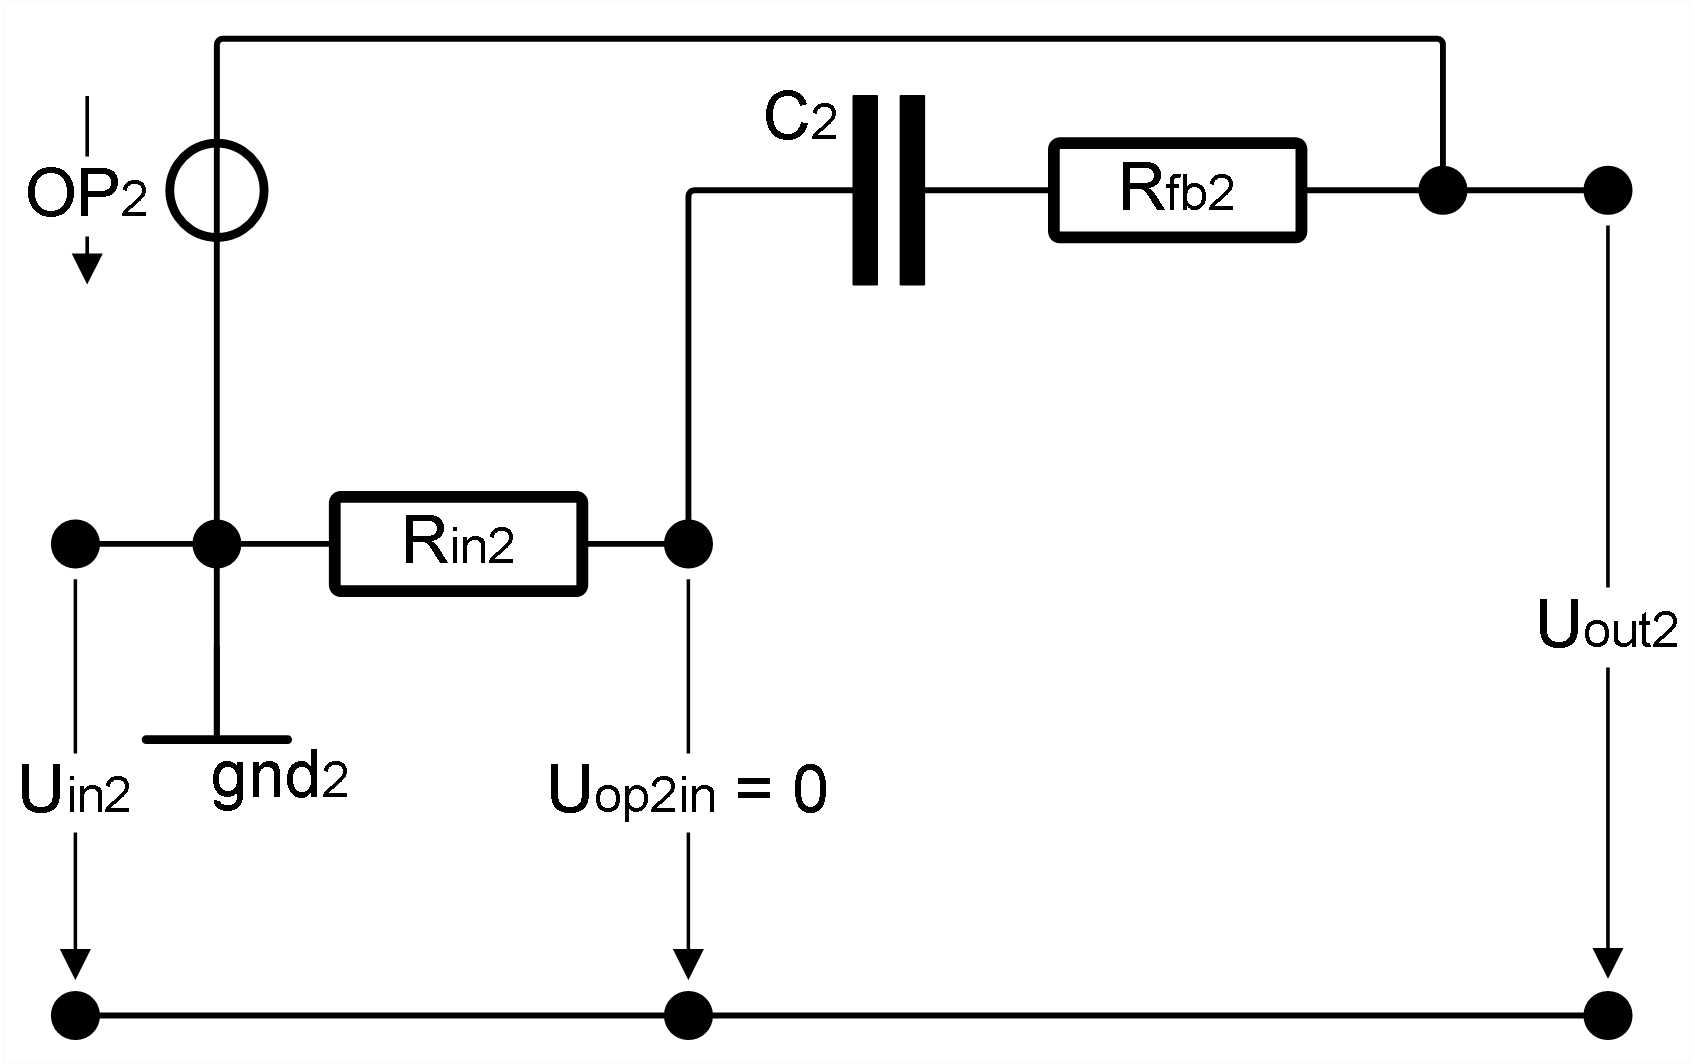
\includegraphics[width=5.96cm]{OpampLPWithDifferingGnds_equivalent}
\caption{Internal, computed model of low-pass filter 2}
\label{figOpampLPWithDifferingGnds_equivalent}
\end{center}
\end{figure}

However, the input impedance (i.e. the transfer function $Z$ from
$I\left(U_{in}\right)$ to $U_{in}$) differs significantly. Variant $1$ of
the filter yields $R_{in}$, which is what we expect but variant $2$ has an
input impedance of infinite (represented by $\frac{1}{0}$ in the result
log). The infinite input impedance is explained by schematic
\ref{figOpampLPWithDifferingGnds_equivalent} that shows how \linnet{}
models the op-amp in this case. The input connectors are open ended and no
current will ever flow into the circuit; this is the meaning of an
infinite input impedance.

It gets even more confusing if we define the node between resistor and
capacitor in the feedback line to be the ground node, please refer to
figure \ref{figOpampLPWithDifferingGnds_variant3}. The controlled voltage
source in \linnet{}'s internal model of the op-amp now doesn't have any
impact on the op-amp's input voltage; the current it can drive only flows
through the resistor in the feedback line. The equation that the op-amp's
input voltage needs to be null can't be fulfilled, the system determinant
is null and the computation fails with error message.

Last but not least the chosen modelling of the op-amp implies that the
output of the op-amp must not be connected to a ground node or to the
output of another op-amp; the controlled voltage source would be
short-circuited in the first case and the system would be underdetermined
in the latter.

An op-amp in the netlist adds a new unknown to the linear equation
system. It is the current flowing from the ground node through the device
and out of its output. The name of this unknown is derived from the name
of the op-amp, the prefix \ident{I\_} is added. 

The new unknown current means a new column in the LES. It contains null
coefficients anywhere but in the row that holds the current balance
of the op-amp's output node. Here, the unknown current is influent and a
one appears as coefficient.

The additional unknown comes along with the new equation $U_{in_1} -
U_{in_2} = 0$. This equation means a row, which has just a pair of $\pm 1$
coefficients at the columns, which are related to the two input node's
voltage potentials (and hence only a single signed one if one of these
nodes is the ground node).

As an example, an op-amp \ident{OP} is connected with its two inputs and
its output to the nodes $N_2$, \ident{GND} and $N_1$, respectively, of the
circuit fragment in figure \ref{figLESCreation_fragmentOfPassiveDevices}.
The new unknown current \ident{I\_OP} is put to the right of the unknowns
so far. The LES would be extended to:

\begin{displaymath}
\left(
\begin{array}{cccccc}
-C      & C      &  0     & \ldots & 1      & \ldots \\
 C      & -C-L-R &  L     & \ldots & 0      & \ldots \\
 0      &    L   & -L     & \ldots & 0      & \ldots \\
 \vdots & \vdots & \vdots &        & \vdots & \ddots \\
 0      & 1      & 0      & \ldots & 0      & 0      \\
\end{array}
\right)
\end{displaymath}


\subsection{Symbols, knowns and unknowns}

The op-amp is ideal and doesn't have a device constant or value. It neither
adds a known to the LES nor a symbol to the computation.

The output current current of the op-amp is a new unknown of the linear
equation system. The name of this unknown is derived from the name of the
op-amp, the prefix \ident{I\_} is added. It can be referenced from a
result definition.


% Same op-amp LP, here with third choice of gnd node
{
% This define is related to the specifics of the array package; see
% http://texwelt.de/wissen/fragen/3401/zentrieren-text-in-tabelle (as of
% July 25 2014) for more
\newcolumntype{M}[1]{>{\centering\arraybackslash}m{#1}}

\begin{figure}[t]
\begin{center}
\begin{tabular}{M{6.5cm}M{5.96cm}}
\verbatiminput{OpampLPWithDifferingGnds_variant3.cnl}
&
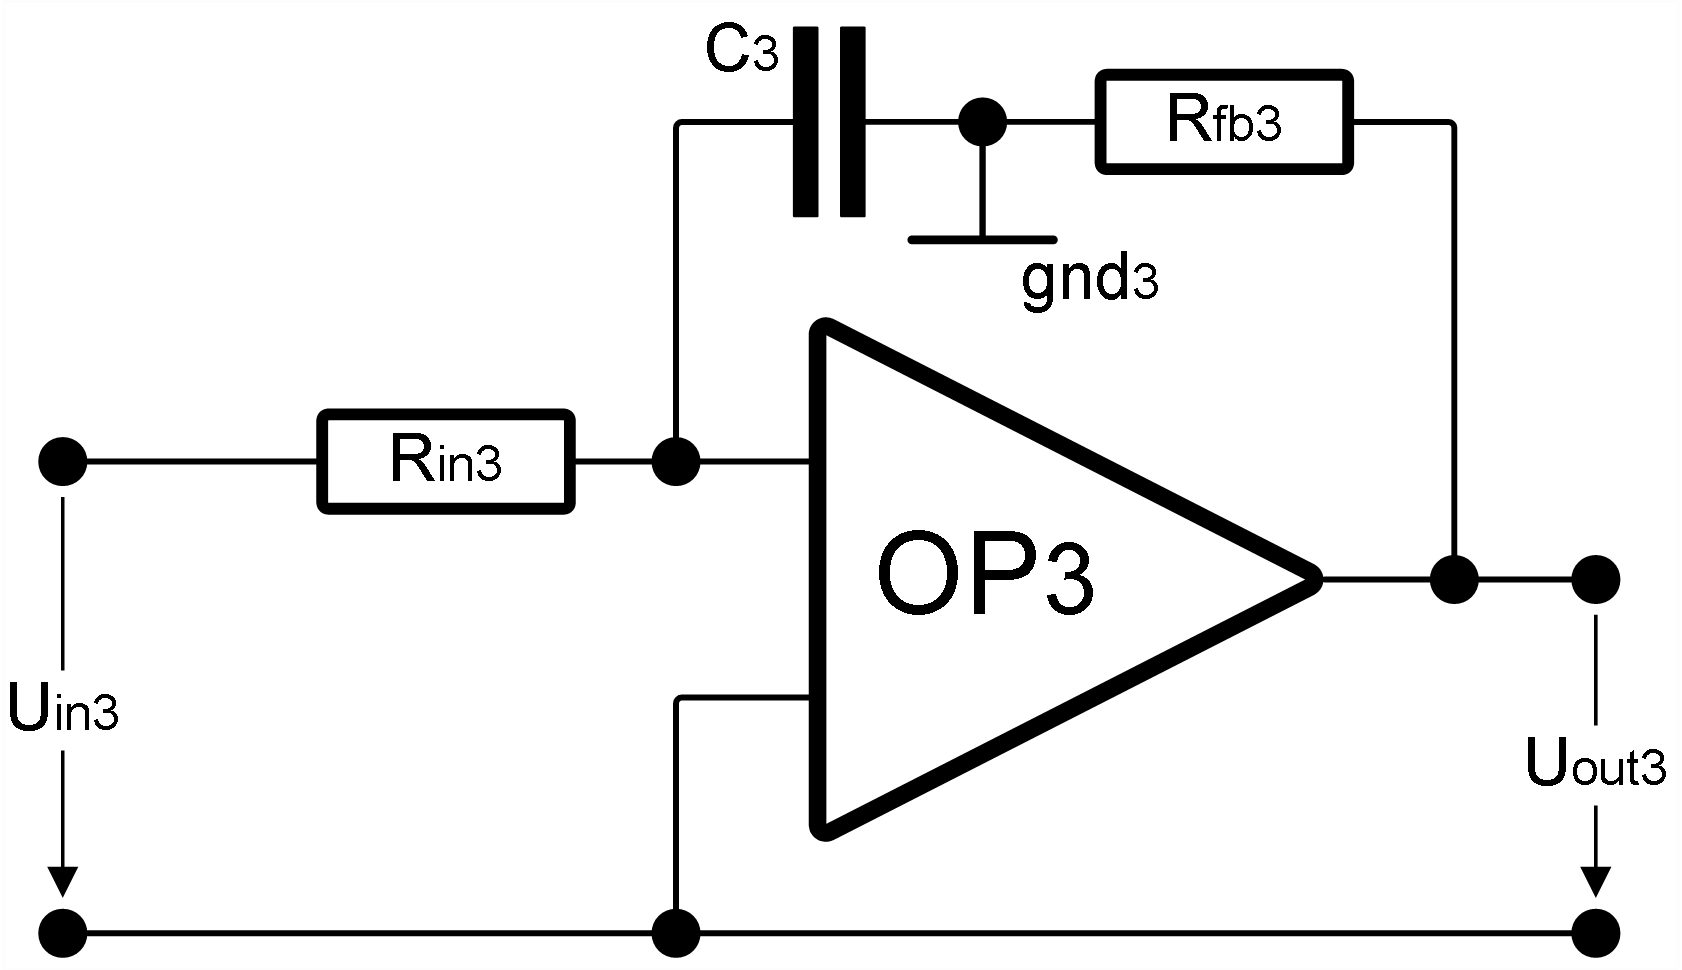
\includegraphics[width=5.96cm]{OpampLPWithDifferingGnds_variant3}

\end{tabular}
\caption{Same low-pass filter with invalid third choice of ground node}
\label{figOpampLPWithDifferingGnds_variant3}
\end{center}
\end{figure}
} % Same op-amp LP, here with third choice of gnd node


\section{Voltage controlled voltage source}

The voltage controlled voltage source is modeled by an additional
equation. The source is connected to two nodes. These node's voltage
potentials, which are both unknowns to the system are associated by the
constraint that they differ by a constant multiple $k$ of a voltage, which
is unknown but which can be expressed as difference of two nodes. The
multiple $k$ is the device constant and is a new symbol in the
computation.

The additional equation is $U_{n_i} - U_{n_j} - kU_{n_u} + kU_{n_v} = 0$;
the voltage source is connected to nodes $n_i$ and $n_j$, $k$ is its
dimensionless device constant and the control voltage is the voltage
potential difference between the nodes $n_u$ and $n_v$.
 
The additional equation means a further row to the LES, which has all null
coefficients but a pair of $\pm 1$ and a pair of $\pm k$. (Both pairs can
reduce to a single signed one or $k$ if one of the references nodes is a
ground node. If both nodes of the control voltage are the ground node then
the $\pm k$ will even disappear entirely.)

The additional equation comes along with an additional unknown. When
setting up the current balance of the nodes the source is connected to we
have to consider the additional circuit branch, the current flowing
through the source. This current is unknown. It is defined to be the
current flowing out of the source's plus pole, which is the first
connected node. This current is influent and thus positive at the node
connected to the plus pole and affluent or negative at the minus pole's
connected node. We get an additional column in the LES, which has a pair
of $\pm 1$ as only non null coefficients (or a single signed one if one of
the connected nodes would be the ground node).


\subsection{Symbols, knowns and unknowns}

The voltage controlled voltage source doesn't introduce knowns to the
equation system.

The name of the device appears as a symbol in the internal computation and
in the final result. It has the meaning of the source's dimensionless
voltage amplification $k$. The value for $k$ used as default in numeric
post-processing with Octave can be found in table \ref{tabDeviceStdValues}
on page \pageref{tabDeviceStdValues}.

The name of the additional unknown, the current through the source is
derived from the device name by adding the prefix \ident{I\_} to the left
of the user-defined device name. This name does not appear as a symbol in
the internal computation. It can be referenced in a result specification
in order to get an according transfer function or full result.


\section{Current controlled voltage source}

The current controlled voltage source is modeled by an additional
equation. The source is connected to two nodes. These node's voltage
potentials, which are both unknowns to the system are associated by the
constraint that they differ by a constant multiple $k$ of a current, which
is an unknown of the LES. (It is the unknown current through a current
probe; please refer to section \ref{secModellingDevs_currentProbe} for
details.) The multiple $k$ is the device constant and it is a new symbol
in the computation.

The additional equation is $U_{n_i} - U_{n_j} - k I_c = 0$;
the voltage source is connected to nodes $n_i$ and $n_j$, $k$ is its
device constant and $I_c$ is the control current, an unknown of the LES.

The additional equation means a further row to the LES, which has all null
coefficients but a pair of $\pm 1$ (or a single signed one if one of the
connected nodes would be the ground node) and a single signed $k$.

The additional equation comes along with an additional unknown. When
setting up the current balance of the nodes the source is connected to we
have to consider the additional circuit branch, the current flowing
through the source. This current is unknown. It is defined to be the
current flowing out of the source's plus pole, which is the first
connected node. This current is influent and thus positive at the node
connected to the plus pole and affluent or negative at the minus pole's
connected node. We get an additional column in the LES, which has a pair
of $\pm 1$ as only non null coefficients (or a single signed one if one of
the connected nodes would be the ground node).


\subsection{Symbols, knowns and unknowns}

The current controlled voltage source doesn't introduce knowns to the
equation system.

The name of the device appears as a symbol in the internal computation and
in the final result. It has the meaning of the source's current to voltage
amplification $k$. The value for $k$ used as default in numeric
post-processing with Octave can be found in table \ref{tabDeviceStdValues}
on page \pageref{tabDeviceStdValues}.

The name of the additional unknown, the current through the source is
derived from the device name by adding the prefix \ident{I\_} to the left
of the user-defined device name. This name does not appear as a symbol in
the internal computation. It can be referenced in a result specification
in order to get an according transfer function or full result.


\section{Voltage controlled current source}

The voltage controlled current source is modeled similar to a passive
device. By definition, the current flowing through the voltage controlled
current source is described by $I = k(U_{n_u} - U_{n_v})$, where $k$ is
the device constant, the amplification from voltage to current, and the
control voltage is the voltage potential difference between the referenced
nodes $n_u$ and $n_v$.

This current is considered when setting up the current balance of the two
nodes the source is connected to. It is defined to be the current flowing
out of the second node in the netlist and it is influent and thus positive
at this node. Vice versa, it is flowing back into the source at the first
node in the netlist or affluent or negative at this node. In each of the
two affected rows of the LES we get a pair of $\pm k$ as further addends
of the coefficients of the unknown voltage potentials of the two
referenced control nodes. (If one of the connected nodes is the ground
node or if one of the nodes that define the control voltage is the ground
node then two of the $\pm k$ disappear; if both holds then only a single
signed $k$ remains.) The appearance pattern of symbol $k$ in the LES is
nearly the same as for the passive devices; the only difference is the
possible appearance as a single pair $\pm k$. Neither an additional known,
unknown nor equation is required.


\subsection{Symbols, knowns and unknowns}

The voltage controlled current source neither introduces knowns nor
unknowns to the equation system. In particular, there's no unknown, which
describes the current through the source. If this current is needed in a
user-specified result then a current probe needs to be placed in series
with the source.

The name of the device appears as a symbol in the internal computation and in
the final result. It has the meaning of the source's voltage to current
amplification $k$. The value for $k$ used as default in numeric
post-processing with Octave can be found in table \ref{tabDeviceStdValues}
on page \pageref{tabDeviceStdValues}.


\section{Current controlled current source}

By definition, the current flowing through the current controlled current
source is described by $I = kI_c$, where $k$ is the device constant, the
dimensionless amplification from control to output current, and $I_c$ is
the control current. $I_c$ is the the current through a current probe
device and such a current always is an unknown of the LES. (Please refer
to section \ref{secModellingDevs_currentProbe} for details.)

The current $I$ is considered when setting up the current balance of the
two nodes the source is connected to. It is defined to be the current
flowing out of the second node in the netlist and it is influent and thus
positive at this node. Vice versa, it is flowing back into the source at
the first node in the netlist or affluent or negative at this node. A pair
of $\pm k$ appears in the column of the LES that belongs to the unknown
control current $I_c$ (or a single signed $k$ if one of the connected
nodes is the ground node). Besides null coefficients this column can also
contain the same pattern from other instances of such sources, if they are
controlled by the same unknown current, and it will contain a pair of $\pm
1$ from the referenced current probe itself. If the devices share their
connected nodes then these ones and symbols share the same row, they
become addends of the coefficient of the LES.

Neither an additional known, unknown nor equation is required.


\subsection{Symbols, knowns and unknowns}

The current controlled current source neither introduces knowns nor
unknowns to the equation system. In particular, there's no unknown, which
describes the current through the source. If this current is needed in a
user-specified result then a current probe needs to be placed in series
with the source.

The name of the device appears as a symbol in the internal computation and
in the final result. It has the meaning of the source's dimensionless
current to current amplification $k$. The value for $k$ used as default in
numeric post-processing with Octave can be found in table
\ref{tabDeviceStdValues} on page \pageref{tabDeviceStdValues}.


\section{The current probe}
\label{secModellingDevs_currentProbe}

The current probe is an ideal wire, which connects two nodes. The voltage
potentials of these two nodes become identical. As a kind of side-effect
the current through this wire becomes a new unknown of the LES and can be
queried in result specifications.

Actually, the current probe is a constant voltage source with voltage
null. Please refer to section \ref{secModellingDevs_ConstVoltSrc} to see
how such a source is modeled. The current probe is different in two
aspects: The way, the name of the new unknown is derived from the device
name is different and no additional known (the constant source voltage) is
introduced to the LES since the voltage is null by definition. All
according terms of the result would have to be taken times null anyway.

The polarity of the unknown current through the current probe is defined
as for the current sources: The unknown current is the one, which flows
out of the second connected node into the network and from the network
node, which is mentioned first in the netlist back into the probe. This
sounds counter-intuitive but isn't: This way, the first and second netlist
node mean the start and end of the arrow in the symbol of the current
probe in this order (see table \ref{tabSupportedDevices} on page
\pageref{tabSupportedDevices}).


\subsection{Symbols, knowns and unknowns}

The current probe doesn't introduce a known to the equation system.

Neither in the internal computation and nor in the final result will the
name of the device appear as a symbol.

The name of the additional unknown, the measured current, is basically
derived from the device name by adding the prefix \ident{I\_} to the left
of the user-defined device name -- as usual for the sources. However, if
the device name already starts with the character sequence \ident{I\_} then
this name extension doesn't take place and the name of the unknown current
is identical with the name of the device. This has been decided for
convenience: It's natural to name a current probe like the measured
current but this must not lead to names like \ident{I\_I\_measured}.
Sticking to the common naming pattern would mean to force the user to name
the current probe device only \ident{measured} in this example, which was
a degradation of the readability of the netlist.

The name of the measured current does not appear as a symbol in the
internal computation. It can be referenced in a result specification in
order to get an according transfer function or full result.
